\chapter{Projekt aplikacji}
\label{cha:projektAplikacji}
Rozdział opisuje architekturę systemu w~ujęciu abstrakcyjnym. Nacisk położony jest na schemat działania oraz przedstawienie komponentów aplikacji. Dodatkowo wyjaśniane są pewne podstawowe pojęcia związane z~inżynierią oprogramowania.

%---------------------------------------------------------------------------
\section{Podstawowe przypadki użycia}
\label{sec:podstawowePrzypadkiUżycia}
Aplikacja ,,DAR'' jest z~punktu widzenia funkcjonalności dość prostym systemem. Rysunek~\ref{fig:usecase} prezentuje podstawowe przypadki użycia -- warto mieć jednak na uwadze fakt, że aplikacja została zintegrowana z~zewnętrznym systemem posiadającym silniki decyzyjne i~procesowe, zatem wiele funkcjonalności niepokazanych tutaj, takich jak uruchamianie procesu, ewaluacja decyzji czy monitorowanie wydajności procesów, leży po jego stronie.
\begin{figure}
    \centering
    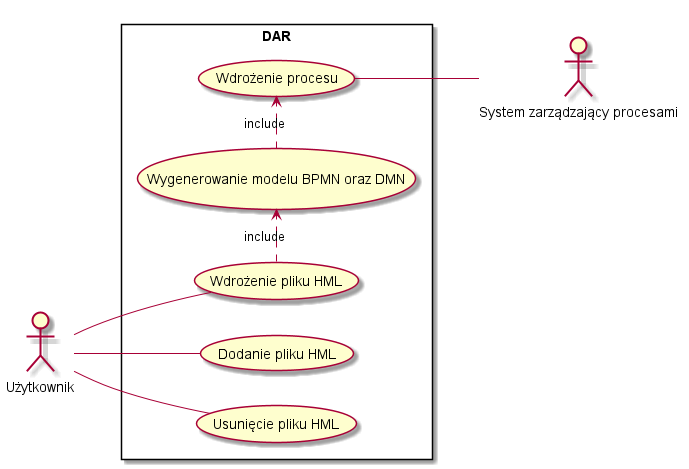
\includegraphics[width=\textwidth, height=0.4\textheight,keepaspectratio]{./assets/usecase.png}
    \caption{Graficzna reprezentacja podstawowych przypadków użycia}
    \label{fig:usecase}
\end{figure} 

Poniżej opisane zostały funkcjonalności zaprezentowane na rysunku~\ref{fig:usecase}:
\begin{itemize}
	\item \textbf{Wdrożenie procesu} -- aplikacja przesyła dwa pliki do zewnętrznego systemu. Pierwszy z~nich to plik reprezentujący proces w~notacji \emph{BPMN}, natomiast drugi to plik reprezentujący diagram decyzji w~notacji \emph{DMN}.
	\item \textbf{Wygenerowanie modelu BPMN oraz DMN} -- aplikacja na podstawie dostarczonych danych generuje dwa modele -- model w~notacji \emph{BPMN} oraz model w~notacji \emph{DMN}. Jednocześnie spaja te dwa modele poprzez odpowiednie ustawienia atrybutów.
	\item \textbf{Wdrożenie pliku HML} -- aplikacja przesyła wybrany plik \emph{HML} i~rozpoczyna proces jego przetwarzania aby finalnie przesłać go do odrębnego systemu procesowego. 
    \item \textbf{Dodanie pliku HML} -- aplikacja zapisuje informację z~plików \emph{HML}.
    \item \textbf{Usunięcie pliku HML} -- aplikacja usuwa wszystkie zapisane informacje z~danego pliku \emph{HML}.
    \item \textbf{Uruchamianie procesu, ewaluacja decyzji, monitorowanie procesu...} -- wiele funkcjonalności nie należy stricte do ram aplikacji ,,DAR'', jednak poprzez integrację z~zewnętrznym systemem, aplikacja pośredniczy w~umożliwianiu takich działań, jak uruchamianie i~śledzenie procesu, edycja tabel decyzyjnych, uzupełnianie danych czy ewaluacja decyzji. 
\end{itemize}

%---------------------------------------------------------------------------
\section{Architektura systemu}
\label{sec:architekturaSystemu}

%---------------------------------------------------------------------------
\subsection{Architektura N-tier}
\label{sec:architekturaNTier}
Aplikacja ,,DAR'' została oparta na architekturze wielowarstwowej zwanej również architekturą N-tier. Jest to jedna z metod tworzenia oprogramowania, opierająca się na wydzieleniu warstw aplikacji -- w~sensie fizycznym oraz logicznym. Warstwy są narzędziem do odseparowania obowiązków\footnote{Jest to ściśle związane z~zasadą SoC (\emph{Separation of Concerns}), czyli podstawową zasadą inżynierii oprogramowania, stanowiącą o tym, że każda część systemu powinna mieć silnie określone granice i~adresować dokładnie odseparowaną kwestię.} danych rejonów aplikacji oraz do zarządzania zależnościami. Każda warstwa posiada konkretną odpowiedzialność. Warstwy wyższe mogą używać usług z~warstw niższych, jednak nie działa to w~drugą stronę. Architektura wielowarstwowa może być:
\begin{itemize}
    \item \textbf{Zamknięta} -- tak jak jest to w~przypadku opisywanego systemu. Dana warstwa może używać jedynie warstwy pod sobą.
    \item \textbf{Otwarta} -- dana warstwa może używać dowolnej warstwy pod sobą.
\end{itemize}

,,DAR'' posiada trzy logiczne warstwy, zaprezentowane na rysunku~\ref{fig:layerExample}.
\begin{figure}
    \centering
    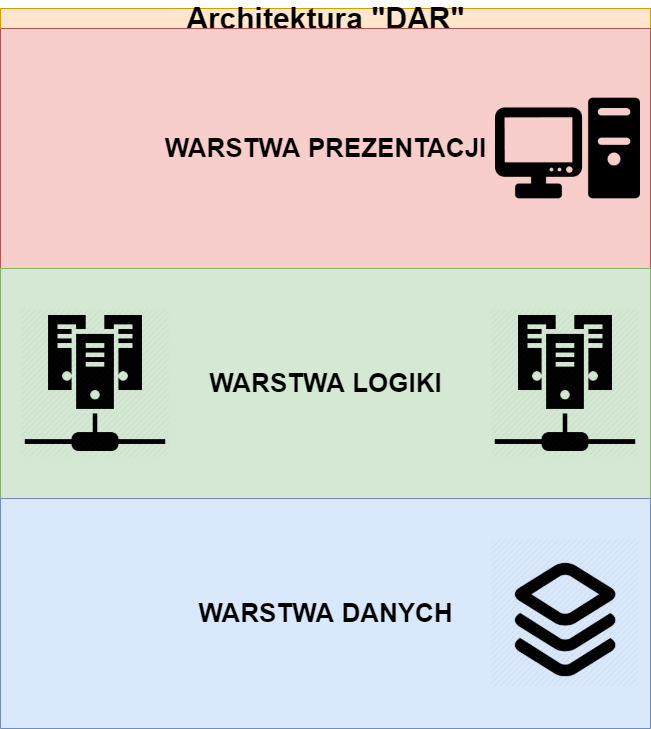
\includegraphics[width=0.4\textwidth,height=0.4\textheight,keepaspectratio]{./assets/layerExample.png}
    \caption{Warstwy aplikacji ,,DAR''}
    \label{fig:layerExample}
\end{figure} 
Poniżej przedstawiony został opis wydzielonych warstw:
\begin{itemize}
    \item \textbf{Warstwa prezentacji} -- najwyższa warstwa. Jej zadaniem jest wyświetlanie danych i~komunikacja z~warstwą niżej. Reprezentuje ona interfejs użytkownika i umożliwia interakcję z~systemem.
    \item \textbf{Warstwa logiki} -- zwana również logiką biznesową, jest to główna część aplikacji, w~której zaimplementowane zostały wszystkie funkcjonalności. W przypadku ,,DAR'' do dyspozycji są tutaj dwa serwisy, jeden będący serwerem ,,DAR'', natomiast drugi to zintegrowany zewnętrzny system do obsługi procesów. Warstwa ta przetwarza dane i~przekazuje je do warstwy prezentacji. 
    \item \textbf{Warstwa danych} -- warstwa związana z~dostępem do danych. W~przypadku ,,DAR'' jest to dostęp do relacyjnej bazy danych, gdzie przechowywane są informacje na temat dodanych plików \emph{HML}. Udostępnia ona dane dla warstwy logiki biznesowej.
\end{itemize}
Zaletami takiego rozwiązania są:
\begin{itemize}
    \item \textbf{Skalowalność} -- dzięki oddzieleniu odpowiedzialności bardzo łatwo zdiagnozować, gdzie aplikacja potrzebuje usprawnień i~co najważniejsze, można to robić tylko w~jednym konkretnym obszarze, co daje o wiele więcej możliwości skalowania.
    \vspace{-1mm}
    \item \textbf{Luźne powiązania} -- architektura wymusza na programiście ograniczenie zależności, dzięki czemu zmiany w~danej warstwie są bezbolesne z~punktu widzenia innych warstw.
    \vspace{-1mm} 
    \item \textbf{Bezpieczeństwo} -- podział na warstwy niesie też ze sobą więcej możliwości ochrony przed atakami, ponieważ w~każdej warstwie może występować inna metoda ochrony. Dodatkowo tak samo jak w~przypadku skalowania można odpowiednio poświęcić środki na ochronę tylko newralgicznych punktów aplikacji (przykładem może być zwiększona ochrona warstwy logiki biznesowej oraz danych niż warstwy prezentacji).
    \vspace{-1mm}
    \item \textbf{Łatwiejszy proces tworzenia aplikacji} -- każdą warstwą może zajmować się inna osoba lub zespół, ze względu na luźne powiązania.
    \vspace{-1mm}
    \item \textbf{Większy nacisk na powtórne użycie} -- dzięki modularności tego podejścia, komponenty są raczej projektowane w~sposób generyczny, co ułatwia ich ponowne użycie.
\end{itemize}

%---------------------------------------------------------------------------
\subsection{Architektura klient-serwer}
\label{sec:architekturaKlientSerwer}
,,DAR'' jest aplikacją internetową działająca na zasadzie klient-serwer. Jest to metoda działania, która opiera się na podzieleniu aplikacji na dwie części i~na komunikacji tych modułów:
\begin{itemize}
    \item \textbf{Front-end} -- część kliencka, działająca na oprogramowaniu klienckim, w~tym przypadku jest to przeglądarka użytkownika. Ta część reprezentuje interfejs użytkownika. W aplikacji ,,DAR'' \emph{front-end} został zrealizowany w~formie SPA (\emph{Single Page Application}\footnote{Więcej na temat \emph{SPA} w~rozdziale \ref{sec:spa}.}). Do tej części należy \emph{warstwa prezentacji} opisywana wcześniej.
    \item \textbf{Back-end} --  część serwerowa, działająca na osobnym serwerze. Do niej należą \emph{warstwa logiki biznesowej} oraz \emph{warstwa danych}  opisane wcześniej. W przypadku systemu ,,DAR'' została zrealizowana za pomocą internetowego \emph{REST}\footnote{Więcej na temat protokołu \emph{REST} w~rozdziale \ref{sec:rest}.} API (\emph{Application Programming Interface}). 
\end{itemize}
 W opisywanej aplikacji klient wysyła zapytanie \emph{HTTP}\footnote{Więcej na temat protokołu \emph{HTTP} w~rozdziale \ref{sec:http}.} przez sieć internetową do serwera, a~ten przetwarza żądanie i~zwraca odpowiedź, często z~towarzyszącymi temu danymi. Komunikacja jest asynchroniczna, dzięki temu zwiększona jest odczuwalna szybkość działania aplikacji.

%---------------------------------------------------------------------------
\subsubsection{Protokół HTTP}
\label{sec:http}
Protokół \emph{HTTP} (\emph{Hypertext Transfer Protocol}) to bezstanowy protokół do przesyłania dokumentów typu hypermedia. Określa on zasady wymiany informacji, normalizuje i~ujednolica sposoby komunikacji pomiędzy urządzeniami. Jego głównym zastosowaniem jest umożliwienie komunikacji pomiędzy aplikacjami internetowymi (przeglądarkami), a~serwerami (komputerami/chmurą). Wymiana informacji przebiega w~następujący sposób:
\begin{itemize}
    \item Klient (przeglądarka) wysyła zapytanie \emph{HTTP} do sieci.
    \item Serwer internetowy otrzymuje zapytanie.
    \item Serwer uruchamia aplikację, aby przetworzyć zapytanie.
    \item Serwer zwraca odpowiedź \emph{HTTP} to przeglądarki.\
    \item Klient otrzymuje odpowiedź.
\end{itemize}
Rysunek~\ref{fig:httpExample} obrazuje wymianę informacji w~protokole \emph{HTTP} pomiędzy klientem a~serwerem,.
\begin{figure}
    \centering
    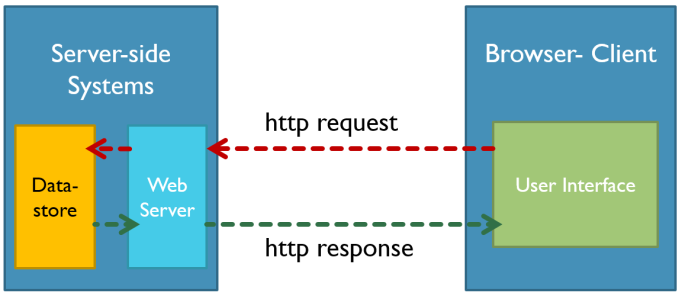
\includegraphics[width=0.5\textwidth,height=0.5\textheight,keepaspectratio]{./assets/httpRequestExample.png}
    \caption{Przykład komunikacji za pomocą protokołu \emph{HTTP}~\cite{HTTP}}
    \label{fig:httpExample}
\end{figure}

Klient, aby otrzymać odpowiedź od serwera, musi określić jego adres oraz metodę określającą jakiego typu jest zapytanie. Najważniejsze metody określone przez specyfikację \emph{HTTP}~\cite{HTTPSpecification} są następujące:
\begin{itemize}
    \item \textbf{GET} -- pobranie zasobu wskazanego za pomocą adresu.
    \item \textbf{PUT} -- wysłanie danych, najczęściej aby zaktualizować pewne istniejące już dane.
    \item \textbf{POST} -- wysłanie danych, najczęściej aby stworzyć kompletnie nowy zasób.
    \item \textbf{DELETE} -- usunięcie danych.
\end{itemize}

%---------------------------------------------------------------------------
\subsubsection{REST API}
\label{sec:rest}
REST (\emph{Representational State Transfer}) jest to styl architektury oprogramowania, bazujący na zbiorze określonych reguł, które określają, jak definiowane są zasoby, a~co za tym idzie, jak można otrzymać do nich dostęp. API (\emph{Application Programming Interface}) jest to zestaw pewnych zasad określających komunikację pomiędzy oprogramowaniem komputerowym. Innymi słowy, wiążąc te dwa pojęcia, \emph{API} to reguły określające, jakie zasoby są dostępne i~jak interesariusz może je uzyskać, natomiast \emph{REST} to styl określający schemat oraz budowę \emph{API}. Aby interfejs był w~pełni zgodny z~\emph{REST}, czyli był \emph{RESTful}, musi spełnić sześć podstawowych reguł z~nim związanych:
\begin{itemize}
    \item \textbf{Klient-serwer} -- system powinien wspierać architekturę typu klient-serwer, jest to związane z~podziałem odpowiedzialności. Odseparowując interfejs użytkownika od przechowywania danych zwiększona zostaje modularność, przez co zyskuje na tym skalowalność.
    \item \textbf{Bezstanowość} -- każda komunikacja na kanale klient-serwer jest w~pełni samowystarczalna, posiada wszelkie niezbędne informacje. Żaden kontekst klienta nie jest przechowywany na serwerze pomiędzy zapytaniami.
    \item \textbf{Zdolność wykorzystania cache'a} -- odpowiedź z~\emph{REST API} musi być jasno określona jako zdolna lub niezdolna do wykorzystania cache'a.
    \item \textbf{Zunifikowany interfejs} -- punkt końcowy, czyli adres danego zasobu powinien być jednoznaczny. Użytkownik zawsze powinien wiedzieć do jakiego zasobu się odwołuje. Polega to głównie na odpowiedniej budowie adresów.
    \item \textbf{System warstwowy} -- system powinien wprowadzać separację warstw.
    \item \textbf{Kod na żądanie} -- zasada opcjonalna polegająca na udostępnianiu klientowi apletów i~skryptów.
\end{itemize}

Główną kwestią, na którą kładzie nacisk \emph{REST} są zasoby. Każda informacja, która może być nazwana, może być zasobem. Zasób jest to obiekt z~typem, danymi, relacjami do innych zasobów oraz z~zestawem metod pozwalających na nim operować. Można go przyrównać do obiektu w~programowaniu obiektowym. Zasoby mogą być oczywiście grupowane w~kolekcję. Stan danego zasobu w~dowolnym czasie jest znany jako reprezentacja zasobu. Zawiera ona dane, metadane opisujące zasób oraz linki typu hypermedia, które pomagają w~podejmowaniu kolejnych akcji. Jeśli chodzi o same dane, które zawiera reprezentacja, przeważnie reprezentowane są one w~formacie \emph{JSON}\footnote{Więcej na temat \emph{JSON}: \url{https://www.json.org/json-en.html}.} (jednak występuje tutaj pełna dowolność, nic nie stoi na przeszkodzie, aby użyć formatu \emph{XML}). 

Mówiąc o metodach, które zasób udostępnia, należy wrócić do wcześniej opisanego protokołu \emph{HTTP}, ponieważ to właśnie tego protokołu używa \emph{REST} do komunikacji. Konsumenci \emph{API} uzyskują dostęp do zasobów poprzez wykorzystanie odpowiedniego internetowego adresu \emph{URI} (\emph{Uniform Resource Identifier}\footnote{Więcej na temat \emph{URI}: \url{https://www.w3.org/Addressing/URL/uri-spec.html}.}) oraz odpowiedniej metody \emph{HTTP}. Innymi słowy komunikacja opiera się na wysyłaniu zapytania \emph{HTTP} z~określoną metodą, pod odpowiedni adres i~otrzymaniu odpowiedzi \emph{HTTP} z~określonym rezultatem i~towarzyszącą mu reprezentacją zasobu. Głównie wykorzystywane są cztery metody, przez co wiele prostych aplikacji będących \emph{RESTful} jest nazywanych aplikacjami \emph{CRUD} -- rysunek~\ref{fig:crudExample} tłumaczy znaczenie tego terminu i~przedstawia wspomniane metody. 
\begin{figure}
    \centering
    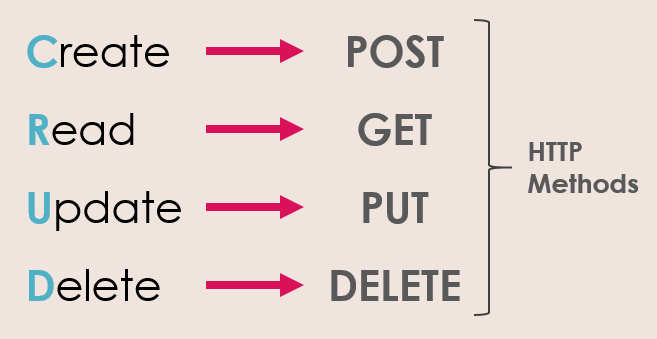
\includegraphics[width=0.5\textwidth,height=0.5\textheight,keepaspectratio]{./assets/crudExample.png}
    \caption{Główne metody wykorzystywane w~\emph{REST API} i~geneza terminu \emph{CRUD}~\cite{CRUD}}
    \label{fig:crudExample}
\end{figure}

%---------------------------------------------------------------------------
\subsubsection{SPA}
\label{sec:spa}
\emph{SPA} (\emph{Single Page Application}) to podejście do tworzenia klienckiego interfejsu użytkownika w~przeglądarce, a~dokładniej wcześniej wspomnianego już front-endu, bardzo mocno zyskujące na popularności w~ostatnich latach, opierające się na dynamicznym wyświetlaniu danych i~przebudowie tylko części widoku. W podejściu klasycznym czyli \emph{MPA} (\emph{Multipage Application}) za każdym razem, kiedy użytkownik nawigował się po stronie internetowej, przeglądarka wysyłała żądanie do serwera i~w~odpowiedzi otrzymywała nową stronę \emph{HTML}\footnote{Więcej na temat \emph{HTML}: \url{https://developer.mozilla.org/pl/docs/Web/HTML}.}, którą następnie wyświetlała. \emph{SPA} inaczej podchodzi do tematu nawigacji, zamiast zawsze prosić o nową stronę \emph{HTML}, cały front-end jest ładowany do przeglądarki na samym początku uruchomienia strony, a~wszelkie zapytania do serwera skutkują jedynie zwróceniem konkretnych danych (najczęściej w~formacie \emph{JSON}). Dzięki temu, to po stronie klienckiej leży odpowiedzialność za odpowiednie wyświetlanie danych. Innymi słowy nie następuje przekierowanie na kolejną stronę, wyświetlana jest cały czas tylko jedna (co zresztą sugeruje nazwa \emph{SPA}), ale to co na niej się znajduje jest dynamicznie zmieniane. 

Warstwa prezentacji w~opisywanej aplikacji została stworzona właśnie w~podejściu \emph{SPA}. Front-end komunikuje się z~serwerem za pomocą \emph{REST API}, otrzymując w~odpowiedzi dane w~formacie \emph{JSON}, a~następnie odpowiednio je przetwarza. Korzyści jakie przynosi ze sobą takie podejście są następujące:
\begin{itemize}
    \item \textbf{Wydajność} -- aplikacja jest szybsza, ponieważ o wiele mniej danych zostaje przetransportowane przez sieć internetową.
    \item \textbf{Mniejsze obciążenie serwera} -- serwer może skupić się tylko i~wyłącznie na przetwarzaniu danych, a~nie na konstrukcji widoku.
    \item \textbf{Większe możliwości prezentacji treści} -- przez brak ciągłego odświeżania strony, umożliwione są efekty, które wcześniej zarezerwowane były jedynie dla aplikacji natywnych dla urządzeń mobilnych lub desktopowych.
    \item \textbf{Zwiększenie odczuwalnej szybkości działania aplikacji} --  aplikacja sprawia wrażenie szybszej, ponieważ niepotrzebne są całościowe przeładowania strony.
\end{itemize}

%---------------------------------------------------------------------------
\section{Schemat projektu}
\label{sec:schematAplikacji}
Rysunek~\ref{fig:projectScheme} przedstawia generalny schemat projektu.
\begin{figure}
    \centering
    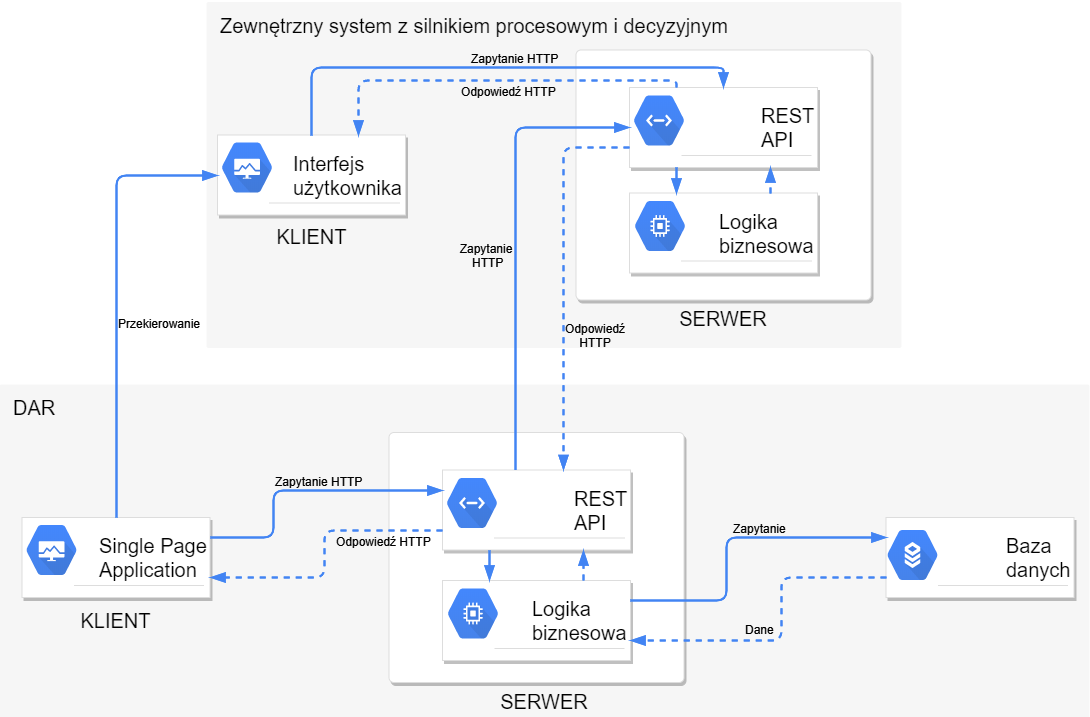
\includegraphics[width=\textwidth]{./assets/projectScheme.png}
    \caption{Schemat projektu ,,DAR''}
    \label{fig:projectScheme}
\end{figure}
Jak widać w~projekcie dochodzi do integracji dwóch systemów. ,,DAR'' udostępnia aplikację \emph{SPA} po stronie klienckiej, która komunikuje się z~serwisem za pomocą \emph{REST API}, wysyłając odpowiednie zapytanie \emph{HTTP}. Serwis po otrzymaniu żądania wykonuje zaimplementowaną logikę biznesową, korzystając przy tym z~bazy danych, aby finalnie zwrócić odpowiedź. Ma on również możliwość komunikacji z~serwisem zewnętrznego systemu, który również udostępnia \emph{REST API}. Front-end aplikacji ,,DAR'' ma możliwość przekierowania użytkownika do interfejsu wspomnianego zewnętrznego systemu. 

Podsumowując schemat projektu, występują w~nim dwa zintegrowane ze sobą serwisy, dwa interfejsy użytkownika oraz baza danych. Sercem całego projektu jest back-end aplikacji, ponieważ to on integruje ze sobą resztę modułów i~to on odpowiedzialny jest za pracę związaną z~generacją modeli procesów i~wdrażaniem ich do zewnętrznego systemu.  

%---------------------------------------------------------------------------
\section{Komponenty}
\label{sec:komponenty}
Nawiązując do rysunku~\ref{fig:projectScheme}, warto przyjrzeć się bliżej części ,,DAR''. Rysunek~\ref{fig:components} prezentuje wyodrębnione komponenty aplikacji. Należy jednak zaznaczyć, że jest to zbliżenie tylko na wspomnianą wcześniej część, nie pojawiają się tam elementy zewnętrznego systemu, z~którymi wiele z~tych komponentów jest zintegrowanych. 
\begin{figure}
    \centering
    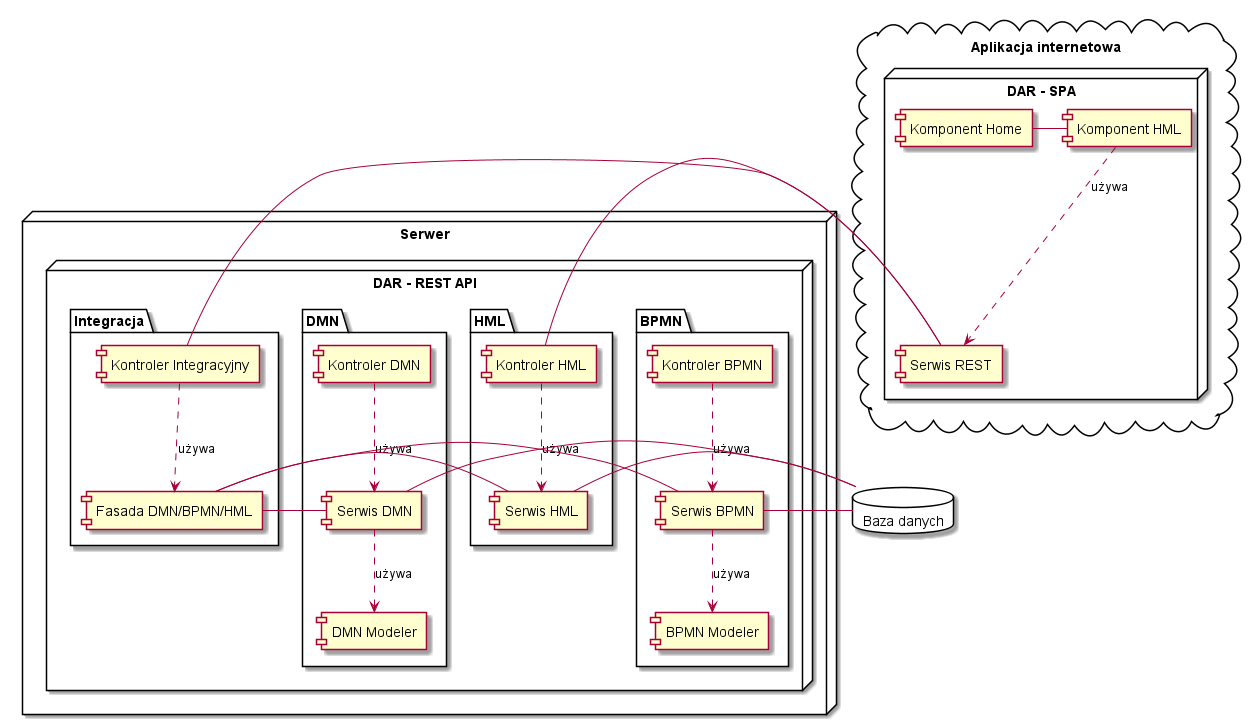
\includegraphics[width=\textwidth]{./assets/components.png}
    \caption{Komponenty aplikacji ,,DAR''}
    \label{fig:components}
\end{figure} 

Podział komponentów na załączonym rysunku jest następujący:
\begin{itemize}
    \item \textbf{Serwer} 
        \begin{itemize}
            \item \textbf{HML}
                \begin{itemize}
                    \item \textbf{Kontroler HML} -- część odpowiedzialna za komunikację \emph{HTTP} i~określająca adresy funkcjonalności związanych z~plikami \emph{HML}.
                    \item \textbf{Serwis HML} -- część odpowiedzialna za logikę biznesową związaną z~plikami \emph{HML}. Zapewnia komunikację z~bazą danych.
                \end{itemize}
            \item \textbf{BPMN}
                \begin{itemize}
                    \item \textbf{Kontroler BPMN} -- część odpowiedzialna za komunikację \emph{HTTP} i~określająca adresy funkcjonalności związanych z~modelami \emph{BPMN}.
                    \item \textbf{Serwis BPMN} -- część odpowiedzialna za logikę biznesową związaną z~modelami \emph{BPMN}. Zapewnia komunikację z~bazą danych.
                    \item \textbf{Modeler BPMN} -- część odpowiedzialna za tworzenie modeli \emph{BPMN}.
                \end{itemize}
            \item \textbf{DMN}
                \begin{itemize}
                    \item \textbf{Kontroler DMN} -- część odpowiedzialna za komunikację \emph{HTTP} i~określająca adresy funkcjonalności związanych z~modelami \emph{DMN}.
                    \item \textbf{Serwis DMN} -- część odpowiedzialna za logikę biznesową związaną z~modelami \emph{DMN}. Zapewnia komunikację z~bazą danych.
                    \item \textbf{Modeler BPMN} -- część odpowiedzialna za tworzenie modeli \emph{DMN}.
                \end{itemize}
            \item \textbf{Integracja}
                \begin{itemize}
                    \item \textbf{Kontroler integracyjny} -- nazwany integracyjnym, ponieważ jego głównym zadaniem jest integracja z~zewnętrznym systemem posiadającym silniki decyzyjne oraz procesowe i~komunikację \emph{HTTP}, określając adresy funkcjonalności związanych z~tym systemem.
                    \item \textbf{Fasada DMN/BPMN/HML} -- fasada wyżej opisanych serwisów, implementująca logikę biznesową związaną z~wdrożeniem modeli procesów do zewnętrznego systemu.
                \end{itemize}
        \end{itemize}
    \item \textbf{Aplikacja internetowa}
        \begin{itemize}
            \item \textbf{Komponent Home} -- część domyślna aplikacji klienckiej, pozwala na nawigację do kolejnych elementów.
            \item \textbf{Komponent HML} -- serce części klienckiej, gdzie znajduje się główny widok i~to on odpowiada za umożliwienie użytkownikowi podstawowych interakcji typu dodanie i~wdrożenie pliku \emph{HML}.
            \item \textbf{Serwis REST} -- serwis do komunikacji za pomocą protokołu \emph{HTTP}, wykorzystywany przez \emph{Komponent HML} do wysyłania zapytań \emph{HTTP}.
        \end{itemize} 
    \item \textbf{Baza danych} -- część odpowiedzialna za przechowywanie danych.
\end{itemize}

%---------------------------------------------------------------------------
\section{Schemat interakcji}
Rysunek~\ref{fig:sequence} prezentuje główny schemat interakcji pomiędzy komponentami na przykładzie procesu wgrywania pliku \emph{HML} przez użytkownika oraz wdrażania tego pliku do zewnętrznego systemu posiadającego silniki decyzyjne oraz procesowe. 

Zaczynając użytkownik dodaje pewien plik, w~założeniu powinien to być plik \emph{HML}. Następnie \emph{Komponent HML} przesyła ten plik poprzez \emph{Serwis REST}. Aplikacja po stronie serwera otrzymuje plik w~\emph{Kontrolerze HML}. Następnie używając \emph{Serwisu HML} tworzy odpowiedni obiekt i~zapisuje go do bazy danych. W przypadku wdrożenia sytuacja początkowa jest podobna -- \emph{Komponent HML} przesyła za pomocą \emph{Serwisu REST} identyfikator odpowiedniego pliku \emph{HML} wraz z~poleceniem wdrożenia. Polecenie trafia do \emph{Kontrolera integracyjnego}, który przekazuje identyfikator do fasady serwisów, która używa \emph{Serwisu HML}. \emph{Serwis HML} pobiera informację o danym pliku identyfikując go dostarczonym identyfikatorem i~zwraca obiekt \emph{HML}. Fasada następnie na podstawie otrzymanego rezultatu używa \emph{Serwisu BPMN} oraz \emph{Serwisu DMN}. Te zwracają odpowiednie modele \emph{BPMN} oraz \emph{DMN}. Fasada po odpowiedzi od serwisów zwraca modele do kontrolera, który komunikuje się z~zewnętrznym systemem wysyłając żądanie wdrożenia otrzymanych z~fasady obiektów. Finalnie komponent po stronie klienckiej, po otrzymaniu pozytywnego rezultatu, przekierowuje użytkownika do zewnętrznego systemu.
\label{sec:schematInterakcji}
\begin{figure}
    \centering
    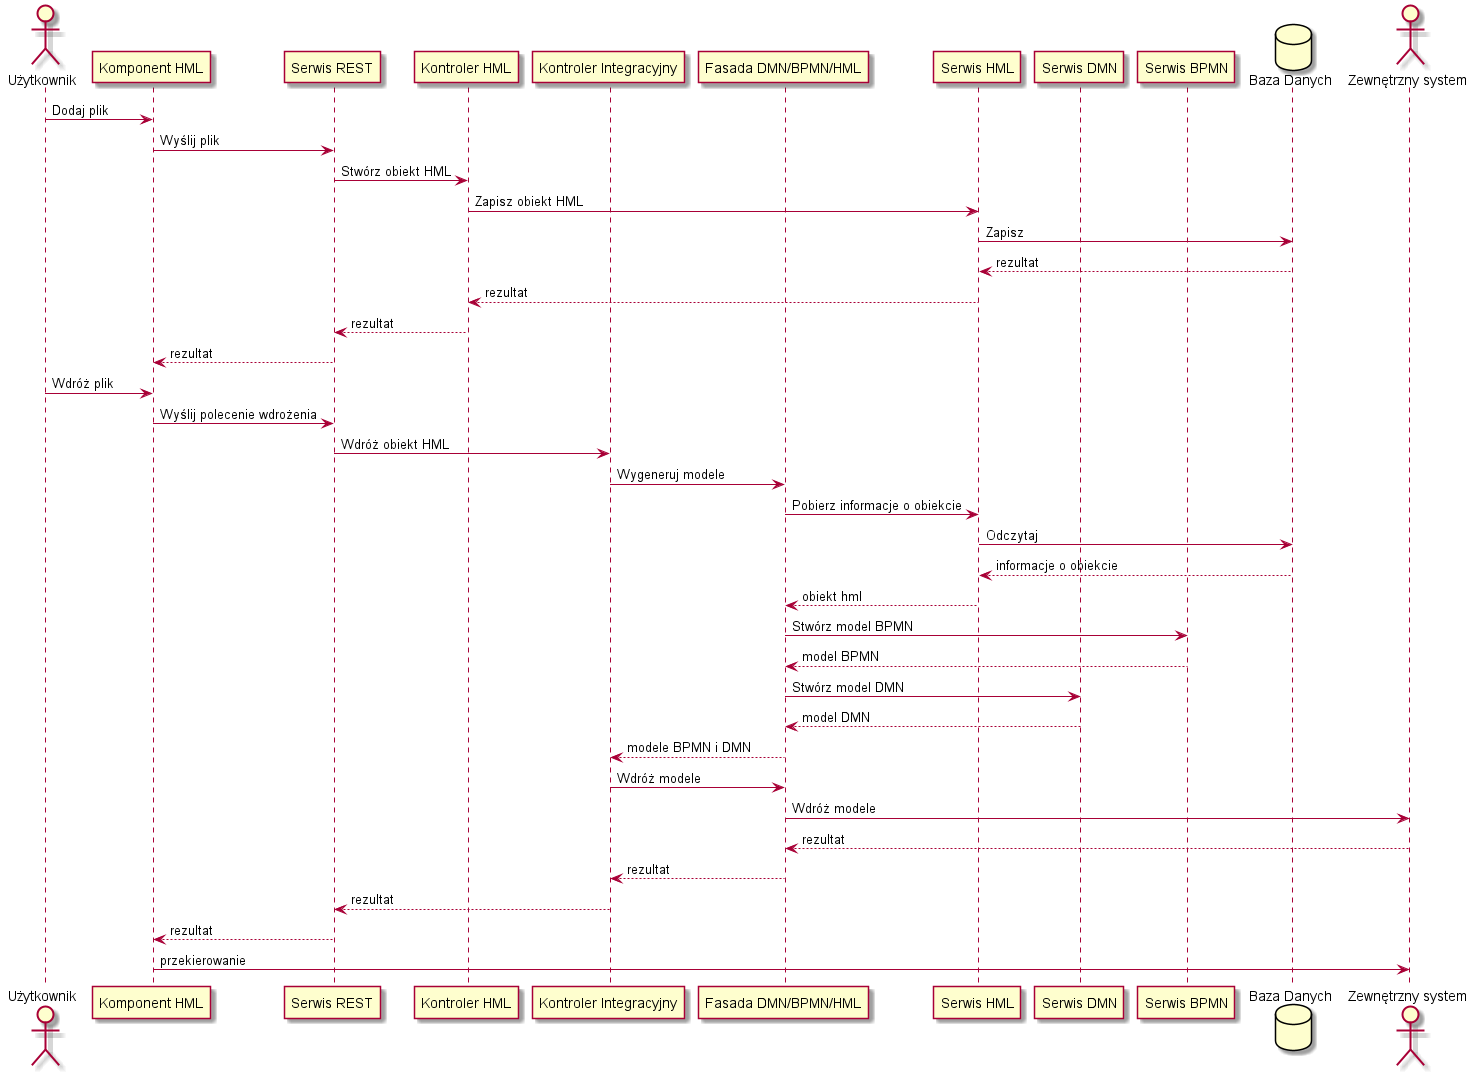
\includegraphics[width=1.4\textwidth, angle=90]{./assets/sequence.png}
    \caption{Schemat interakcji w~aplikacji ,,DAR''}
    \label{fig:sequence}
\end{figure}  
\vspace{1cm}

Jest to koniec rozdziału opisującego projekt aplikacji. W~tym rozdziale została przedstawiona architektura systemu będącego głównym tematem niniejszej pracy. W kolejnym rozdziale zostanie opisana implementacja przedstawionego tutaj projektu, jakie technologie zostały użyte oraz w~jaki sposób zaimplementowane zostały najważniejsze, wspomniane tutaj komponenty aplikacji.



